
\documentclass[12pt,a4paper,titlepage,final]{article}

% cestina a fonty
\usepackage[czech]{babel}
\usepackage[utf8]{inputenc}
% balicky pro odkazy
\usepackage[bookmarksopen,colorlinks,plainpages=false,urlcolor=blue,unicode]{hyperref}
\usepackage{url}
% obrazky
\usepackage[dvipdf]{graphicx}
% velikost stranky
\usepackage[top=3.5cm, left=2.5cm, text={17cm, 24cm}, ignorefoot]{geometry}

\usepackage{mathtools}

\usepackage{alltt}


\begin{document}

%%%%%%%%%%%%%%%%%%%%%%%%%%%%%%%%%%%%%%%%%%%%%%%%%%%%%%%%%%%%%%%%%%%%%%%%%%%%%%
% titulní strana
\begin{titlepage}

% \vspace*{1cm}
\begin{figure}[!h]
  \centering
  
\includegraphics[height=4cm]{img/FIT_barevne_PANTONE_CZ.eps}
\end{figure}

\vfill

\begin{center}
\begin{Large}
Dokumentace k projektu pro předměty IAL a IFJ\\
\end{Large}
\bigskip
\begin{Huge}
Implementace intepretu jazyka IFJ15
\end{Huge}

\end{center}

\vfill

\begin{center}
\begin{Large}
\today
\end{Large}
\end{center}

\vfill

\begin{flushleft}
\begin{large}
\begin{tabular}{ l l l }
Řešitel              & Login & Rozdělení bodů \\
\hline
Jakub Lužný (vedoucí) & xluzny00 & 25\% \\
Jakub Lukáč & xlukac09 & 25\% \\
Viktor Jančík & xjanci09 & 25\% \\
Dušan Litvík & xlitvi01 & 25\% \\
\end{tabular}
\end{large}
\end{flushleft}
\end{titlepage}


%%%%%%%%%%%%%%%%%%%%%%%%%%%%%%%%%%%%%%%%%%%%%%%%%%%%%%%%%%%%%%%%%%%%%%%%%%%%%%
% obsah
\pagestyle{plain}
\pagenumbering{roman}
\setcounter{page}{1}
\tableofcontents

%%%%%%%%%%%%%%%%%%%%%%%%%%%%%%%%%%%%%%%%%%%%%%%%%%%%%%%%%%%%%%%%%%%%%%%%%%%%%%
% textova zprava
\newpage
\pagestyle{plain}
\pagenumbering{arabic}
\setcounter{page}{1}

%%%%%%%%%%%%%%%%%%%%%%%%%%%%%%%%%%%%%%%%%%%%%%%%%%%%%%%%%%%%%%%%%%%%%%%%%%%%%%
\section{Úvod} \label{uvod}
%%%%%%%%%%%%%%%%%%%%%%%%%%%%%%%%%%%%%%%%%%%%%%%%%%%%%%%%%%%%%%%%%%%%%%%%%%%%%%
Táto dokumentácia popisuje implementáciu interpretu imperatívneho jazyka IFJ15. Implementácia je projektom do predmetov \textit{Formální jazyky a překladače} a \textit{Algoritmy}. Úlohou tohoto interpreta je kontrola zdrojového kódu a jeho interpretácia, v prípade, že je zdrojový kód v poriadku. V opačnom prípade dôjde ku chybovému stavu. 

Projekt je možné rozdeliť na niekoľko hlavných celkov:

\begin{itemize}
\item Lexikálný analyzátor – zo zdrojového kódu získavá tokeny.
\item Syntaktický analyzátor – skladá sa z analyzátora jazykových konštrukcií a analyzátora výrazov. 
\item Interpret.
\end{itemize}

Táto dokumentácia má za cieľ popísať proces konštrukcie interpretu z rozdielnych hľadísk. 

\subsection{Rozbor zadania}
Vytvorenie programu v jazyku C, ktorý má fungovať ako interpret jazyka IFJ15, ktorý je podmnožinou jazyka C++11.


Interpret má podporovať nasledujúce dátové typy:

\begin{itemize}
\item string,
\item int,
\item double
\end{itemize}

Samozrejmosťou sú základné aritmetické operácie s uvedenými dátovými typmi. Okrem toho má interpret podporovať vetvenie \texttt{if - else} a cyklus \texttt{for}. Ďalším klúčovým slovom je \texttt{return}. Jednou z nevyhnutných častí akéhokoľvek programovacieho jazyka sú komentáre, náš interpret ich musí podporovať vo forme riadkových komentárov ( \texttt{//} ), ale i vo forme viacriadkových komentárov ( \texttt{/* \ldots */} ). 
Interpret by mal byť chopný spracovať základné aritmetické operátory \texttt{+}, \texttt{-}, \texttt{*}, \texttt{/} ako i relačné operátory \texttt{<}, \texttt{>}, \texttt{>=}, \texttt{<=}, \texttt{==}, \texttt{!=}.
Interpret podporuje modifikátor \texttt{auto}

Naviac  je schopný pracovať so vstavanými funkciami:

\begin{itemize}
\item \texttt{int length (string s)}
\item \texttt{string substr (string s, int i, int n)}
\item \texttt{string concat (string s1, string s2)}
\item \texttt{int find (string s, string search)}
\item \texttt{string sort (string s)}
\end{itemize}

%%%%%%%%%%%%%%%%%%%%%%%%%%%%%%%%%%%%%%%%%%%%%%%%%%%%%%%%%%%%%%%%%%%%%%%%%%%%%%
\section{Implementácia} \label{implementace}
%%%%%%%%%%%%%%%%%%%%%%%%%%%%%%%%%%%%%%%%%%%%%%%%%%%%%%%%%%%%%%%%%%%%%%%%%%%%%%

\subsection{Lexikálný analyzátor}
Lexikálný analyzátor je prvou časťou interpreta, ktorá príde do kontaktu s kódom. Jeho úloha spočíva
v čítaní zdrojového kódu, jeho rozdelenie na lexémy a ich následnú logickú reprezentáciu tzv.
\textit{tokenmi}, ktorí sú výstupmi lex. analyzátoru.

Jednotlilé tokeny obsahujú informácie o type posielaného tokenu, ďalej v závislosti na type
informáciu či sa jedná o aritmetický alebo relačný operátor, v prípade typu string samotný reťazec
a v prípade double alebo int jeho hodnotu.

Nevyhnutnou úlohou lexikálneho analyzátora je odstránenie akýchkoľvek komentárov a bielych
znakov zo zdrojového programu. Lexikálny analyzátor taktiež kontroluje lexikálnu stránku kódu
a odhaluje lexikálne chyby.

Lexikálny analyzátor je implementovaný pomocou konečného automatu, ktorého grafického
interpretácia je zobrazená nižšie. Pre lepšie grafické znázornenie boli do schémy pridané niektoré
stavy, reálne sa nenachádzajúce v zdrovom kóde.

\begin{figure}[]
  \centering
  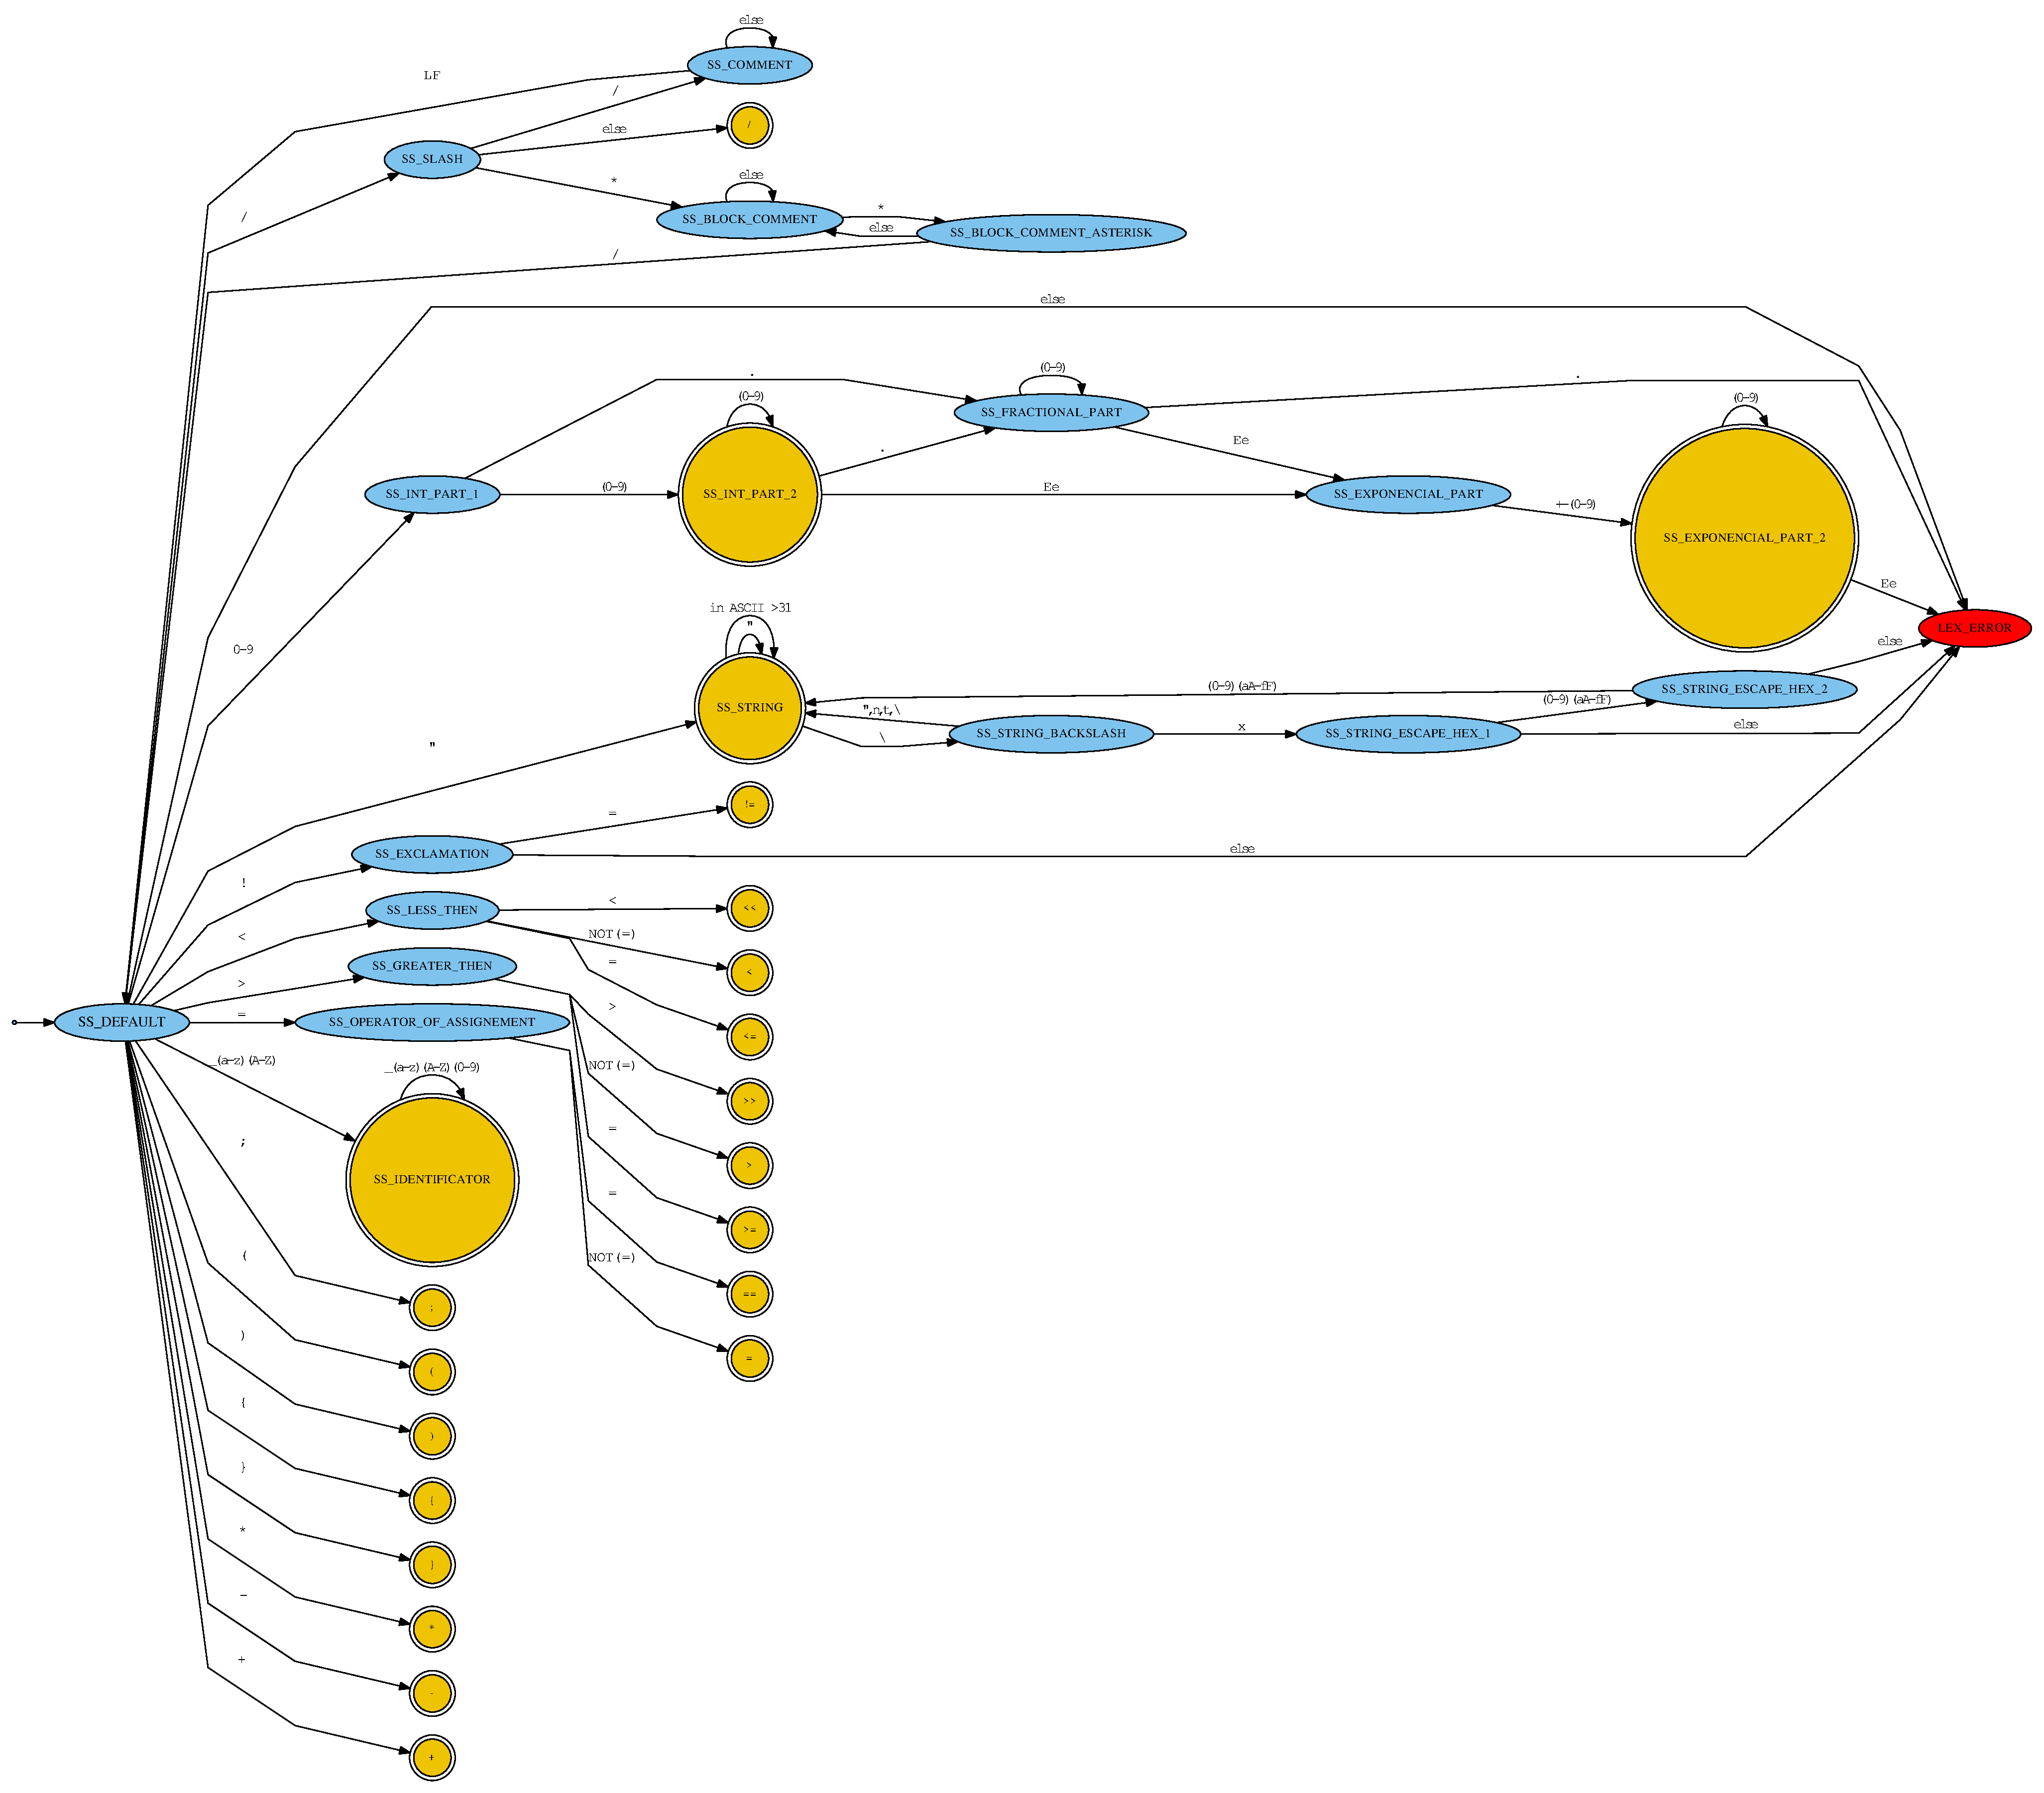
\includegraphics[scale=0.25]{img/fsm.eps}
  \caption{Diagram konečného stavového automatu lexikálního analyzátoru)}
  \label{fig:fsm}
\end{figure}

%=============================================================================
\subsection{Syntaktický a sémantický analyzátor}

Fukčným jadrom interpretu je syntaktický analyzátor. Jednou z úloh je kontrola syntaktickej správnosti programu. Syntax a jej pravidlá sú definované pomocou LL gramatiky, čiže syntaxe jazyka. Ďalej prebieha sémantická kontrola. Úlohou sémantickej kontroly je napr. kontrolovať korektné použitie dátových typov. Hlavnou úlohou syntaktického analyzátora je v prípade správnosti zdrojového programu jeho preklad na postupnosť pseudoinštrukcií. V opačnom prípade dôjde ku syntaktickej chybe.

Analyzátor si pomocou funkcie \verb+token_t get_next_token(scanner* s)+ načíta jednotlivé tokeny (dodávané lexikálnym analyzátorom) zo zdrojového súboru. Tie následne spracováva pomocou metód syntaktickej analýzy a vytvára pseudokód.

V našej implementácií používame dve rôžne tabuľky symbolov. Jedna je globálna tabuľka funkcií, druhá je zásobník tabuliek premenných. So zásobnikom pracujeme tak, že pri vstupe do nového bloku vytvoríme novú tabuľku premenných pre ten blok, a vložíme ju na vrchol zásobníku. Pri odchode z bloku, tabuľku premenných na vrchole zásobníku odstránime a dealokujeme.

Syntaktická analýza prebieha metódou rekurzívneho zostupu a využíva pravidlá LL gramatiky. 

\subsection{LL gramatika}
\begin{alltt}

funcs -> funcHead funcs | EOF
varDef -> auto id = expr | type id varDefFollow
varDefFollow -> = asgnFollow | \(\epsilon\)
type -> int_t | double_t | string_t
funcHead -> type id ( paramSpec ) funcBody
	funcBody -> ; | block
paramSpec -> type id paramSpecFollow | \(\epsilon\)
	paramSpecFollow -> , type id paramSpecFollow | \(\epsilon\)
term -> int | double | string | id
paramList -> term paramListFollow | \(\epsilon\)
	paramListFollow -> , term paramListFollow | \(\epsilon\)
block -> { stmts }
asgn -> id = asgnFollow
asgnFollow -> expr | id ( paramList )
ifClause -> if ( expr ) block else block
forClause -> for ( varDef ; expr; asgn ) block
coutStmt -> cout << term coutStmtFollow
coutStmtFollow -> << term coutStmtFollow | \(\epsilon\) 
cinStmt -> cin >> id cinStmtFollow
cinStmtFollow -> >> id coutStmtFollow | \(\epsilon\)
stmt -> varDef; | asgn; | return expr; | coutStmt; | cinStmt; | block\\ | ifClause | forClause
stmts -> stmt stmts | \(\epsilon\)

\end{alltt}

Vstupný bod syntaktického analyzátora je funkcia \verb+parse_program+, ktorá volá funkciu \verb+parse_funcs+, ktorá slúži ako vstupný bod pre LL gramatiku. Následne pomocou rekurzívnych volaní funkcií \verb+parse_*+, kde \verb+*+ zodpovedá názvom produkcií v LL gramatike. Zároveň s syntaktickou analýzou sa vykonáva sémantická analýza v príslušných funkciách produkcií. Funkcia \verb+parse_expr+ slúží na syntaktickú a sémantickú analýzu výrazov a zároveň ako vstupný bod pre precedenčný syntaktický analyzátor. Zároveň so syntaktickou a sémantickou analýzou sa vykonáva generovanie kódu.

%=============================================================================
\subsection{Precedenčná analýza}

Precedenčná analýza slúži ku vyhodnocovaniu výrazov. Kedykoľvek syntakt. analyzátor narazí v pravidle na výraz, je volaná preced. analýza, ktorá mu následne vracia spracovaný výraz. 

Ku svojej činnosti potrebuje a využíva lexikálny analyzátor, ktorý jej dodáva tokeny. Pri aplikácii precedenčných pravidiel sú priamo generované inštrukcie. Syntaktické pravidlá pre precedenčnú analýzu sú jej základom a spolu s precedenčnou tabuľkou sú zadefinované nižšie. 
\begin{verbatim}
Expression grammar (missing function calls, rel ops)
	expr -> expr < expr | expr > expr | expr <= expr | expr >= expr | expr != expr
	expr -> expr + expr | expr - expr
	expr -> expr * expr | expr / expr
	expr -> ( expr )
	expr -> int | double | string | id
\end{verbatim}

\begin{table}
\begin{center}
\begin{tabular}{ | l | l | l | l | l | l | l | l |  }
\hline
            & \verb+<>=+& \verb;+-; & \verb+*/+ & \verb+(+  & \verb+)+  & \verb+id+ & \verb+$+ \\ \hline
\verb+<>=+  & \verb+>+  & \verb+<+  & \verb+<+  & \verb+<+  & \verb+>+  & \verb+<+  & \verb+>+ \\ \hline
\verb;+-;   & \verb;>;  & \verb;>;  & \verb;<;  & \verb;<;  & \verb;>;  & \verb;<;  & \verb;>; \\ \hline
\verb;*/;   & \verb;>;  & \verb;>;  & \verb;>;  & \verb;<;  & \verb;>;  & \verb;<;  & \verb;>; \\ \hline
\verb;(;    & \verb;<;  & \verb;<;  & \verb;<;  & \verb;<;  & \verb;=;  & \verb;<;  & \verb;E; \\ \hline
\verb;);    & \verb;>;  & \verb;>;  & \verb;>;  & \verb;E;  & \verb;>;  & \verb;E;  & \verb;>; \\ \hline
\verb;id;   & \verb;>;  & \verb;>;  & \verb;>;  & \verb;E;  & \verb;>;  & \verb;E;  & \verb;>; \\ \hline
\verb;$;    & \verb;<;  & \verb;<;  & \verb;<;  & \verb;<;  & \verb;E;  & \verb;<;  & \verb;E; \\ \hline

\end{tabular}
\caption{Precedenční tabulka}
\label{table:prec}
\end{center}
\end{table}

Samotný algoritmus je tvorený, postupným načítavaním jednotlivých tokenov a vykonávaním operácie určenej precedenčnou tabuľkou s využitím zásobníku. Jednotlivé znaky v tabuľke vyjadrujú operácie push(\verb+<+), reduce(\verb+>+), push only(\verb+=+) a nedovolenú kombináciu(\verb+E+). Operácia je z tabuľky vybraná na základe načítaného terminálu a posledného terminálu na zásobníku. Takže dochádza ku postupnému vyhodnocovaniu a redukovaniu symbolov na zásobníku pomocou pravidiel precedenčnej tabuľky. Pre potreby algoritmu bol implementovaný zásobník, ktorý predstavuje pomocnú dátovú štruktúru.


%=============================================================================
\subsection{Interpret}
Úlohou interpretu je vykonávanie programu, zapísaného pomocou pseudoinštrukcií. Interpret postupne lineárne prechádza a vykonáva postupnosť inštrukcií. Ako pomocnú dátovú štuktúru využíva zásobník, kde uchováva potrebné dáta, premenné, medzivýsledky operácií a riadiace hodnoty. Naviac umožňuje aj nelineárny posun vo vektore inštrukcií pomocou skokových inštrukcií. Jazyk IFJ15 umožňuje aj volanie funkcií, z toho dôvodu bolo potrebné implementovať mechanizmus volania ako súčasť interpreteru. Výsledné riešenie vytvorí nový funkčný rámec na zásobníku dát a následne opäť lineárne vykonáva postupnosť pseudoinštrukcií. Pri návrate z funkcie je obnovený funkčný rámec volajúcej funkcie a návratová hodnota je predaná na vrchole zásobníku. Vstupná funkcia do interpretovaného programu je funkcia \texttt{main}, ktorej adresa je počiatočnou adresou pseudoinštrukcie pri začatí vykonávania programu.

%=============================================================================
\subsection{Riešenie vybraných algoritmov}

\subsubsection{Tabuľka symbolov}
Tabuľka symbolov je implementovaná formou hešovacej tabuľky. Tabuľka sa skladá z poľa zretazených zoznamov. Prvok zretazeného zoznamu je \texttt{symbol\_t} ktorý obsahuje všetky potrebné informácie o dannej premennej / funkcií. Ako hešovací algoritmus sme použili modulárne hešovanie. Každý znak v reťazci sa zahešuje ako jeho ASCII hodnota plus 31 * heš kód predošlých znakov v reťazci. Ceľkový heš kód reťazca sa potom dá do rozsahu veľkosti hešovacej tabuľky, pomocou modula veľkostou hešovacej tabuľky. Hešovacia tabuľka sa automaticky zväčsuje keď priemerná dĺžka zretazeného zoznamu nadobudne dĺžku väčšiu ako 5 prvkov za predpokladu uniformného hešovania. Veľkosti hešovacej tabuľky sú vždy prvočísla, aby sa predošlo sitúciam kde heš kód nejakého stringu má spoločný faktor s veľkostou hešovacej tabuľky. Toto opatrenie zlepšuje uniformnosť výsledných hešov. 

\subsubsection{Boyer-Moore}

Tento algoritmus je považovaný za najefektívnejší v bežných aplikáciach. Algoritmus porovnáva vzor s textom sprava doľava, začínajúc prvkom najviac vpravo. Postup v prípade nezhody sa odvíja od použitej heuristiky. V našom projekte sme použili tzv. Bad Character Shift. Táto heuristika si pred vyhľadávaním zostaví tabulku, kde je pre každý znak údaj o tom, ako ďaleko je jeho ďalší najbližší výskyt. Následne sa pri nezhode vždy posunie o tento počet zankov, namiesto jedného ako by to robil naivný algoritmus.  

\subsubsection{Quick-sort}

Ide o radiaci algoritmus s najmenšou priemernou zložitosťou na reálnych dátach. Na začiatku sa taktiež zvolí pivot. Jeho voľba má zásadný vpliv na rýchlosť algoritmu. V ideálnom prípade by sa malo jednať o medián. V našej implementácií sa ako pivot volí prostredný prvok poľa. Podľa tohoto pivota sa pole rozdelí na dve polovice a prvky prehádžeme tak, aby na jednej strane boli menšie ako pivot a na druhej strane naopak väčšie. Tent postup opakujeme pre obidve rozdelené časti (bez pivota, ktorý už je umiestnený na správnom mieste). Procedúru opakujeme až kým nenarazíme na všetky triviálne riešiteľné podproblémy, tzn. pole o veľkosti 1. 

%=============================================================================
\subsection{Popis riešenia}

Pretože na zložitosť projektu a jeho náročnosť na čas, ale i schopnosti sme boli upozornení dopredu, v dostatočnom predstihu sme si zložili tým. Mesiac po začiatku semestra sme si stanovili pravidelné týždenné schôdzky, kde sme riešili vykonanú prácu, analyzovali postup práce a jednotlivé problémy. 

Praktická tvorba kódu prebiehala s využitím verzovacieho nástroja Git, na komunikáciu slúžila uzavretá skupina na Facebook-u. Komunikačný kanál nebol zvolený vhodne, čo sa ukázalo v okamihu keď sa zväčšil objem komunikácie a stala sa neprehľadnou. Následne sme prešli na Slack. Pre potreby zdieľania informácií sme využili Google Docs.

Práca na vybraných jednotlivých častiach projektu prebiehala paralelne, naopak iné časti na seba boli úzko naviazané a s vývojom sa čakalo, resp. vývoj týchto častí mal na starosti jeden človek pre uľahčenie tvorby kódu a celistvosť práce. 

Mnohé časti implementácie boli predmetom diskusií (napr. forma a obsah tokenov predávaných lexikálnym analyzátorom), naopak iné časti boli plne v kompetencii daného člena týmu. 

\subsubsection{Rozdelenie práce}
\begin{description}
  \item[Dušan Litvík] lexikálny analyzátor, dokumentácia
  \item[Jakub Lužný] vstavané funkcie, vedenie projektu
  \item[Jakub Lukáč] syntaktická a sémantická analýza výrazov, interpret
  \item[Viktor Jančík] návrh a implementácia dátových štruktúr, syntaktická a sémantická analýza mimo výrazov
\end{description}

\subsubsection{Metriky kódu}
\paragraph{Počet súborov:} 31
\paragraph{Počet riadkov zdrojového kódu:} 5405
\paragraph{Veľkosť statických dát:} 1204B
\paragraph{Veľkosť spustiteľného súboru:} 85508B

%=============================================================================
\subsection{Záver}
Hoci šlo len o školský projekt, museli sme sa vysporiadať s rovnakými problémami aké sa vyskytujú v každom komerčnom projekte, či lepšie povedané v reálnom prostredí. Stratégia vývojového procesu, medziľudská komunikácia, uchovávanie a zdieľanie informácií a mnoho ďalších problémov nám prinieslo mnoho užitočných skúseností. 

\subsection{Literatúra}
\begin{thebibliography}{Per00}
  \bibitem[IFJop]{ifjop} 
    \emph{Studijní opora IFJ}.
    \bibitem[IFJpr]{ifjpr} 
    \emph{Přednášky IFJ}.
  \bibitem[BM]{homesim}
    \emph{Boyer-Moore algorithm}. (1997).\\
    \verb|http://www-igm.univ-mlv.fr/~lecroq/string/node14.html|
\end{thebibliography}

\end{document}
